\subsection{Cyber-Physical systems}

Inden for Cyber-physical systemer differentierer man mellem funktionelle og ikke-funktionelle krav. Funktionelle krav er krav, der viser \textit{hvad} systemet skal kunne gøre. De beskriver altså en opførsel (metode). De funktionelle krav for systemet kan deles op i de forskellige subsystemer. Desktop-klienten og Rest API'et slås sammen, da disse deler funktionalitet. Desktop-klienten kalder til API'et hvori logikken håndteres, og logik i klienten mindskes derved. EPG Polleren har egne funktionelle krav. Disse krav kan findes i bilag \ref{funktionelle_krav}. Kravene er bl.a fundet ud fra den udleverede projektbeskrivelse, og et møde med TV2 hvor spørgsmål er blevet besvaret. \\

Ikke-funktionelle krav beskriver \textit{hvordan} et system virker. Det kunne fx være hvor lang tid et API kald må tage fra man trykker på knappen til klienten opdateres. Også her deles kravene op i subsystemer. De ikke-funktionelle krav for desktop-klienten kan fx være at brugeren skal have besked om fejl via en popup-boks, eller at ofte brugte knapper skal virke inden for 300 millisekunder. Disse krav kan findes i bilag \ref{ikke-funktionelle_krav}. \\

\\
Ud fra de fundne funktionelle krav kan der udarbejdes EAST-ADL modeller. Disse modeller skal vise hvordan de pågældende subsystemer hænger sammen. Hver model indeholder flere forskellige funktions bokse, der repræsenterer de vigtigste komponenter i systemet, associeret med det enkelte krav. Disse funktionsbokse har relationer der viser hvordan de forskellige subsystemer interagerer med hinanden. Hver funktionsboks repræsenterer henholdsvis en miljø (environment) funktionsboks og en analyse funktionsboks. I EAST-ADL modeller vil analyse funktionsboksen indeholde flere funktionsbokse, og vise interaktionerne herimellem.\\

I figur \ref{fig:main} ses et eksempel på den primære EAST-ADL model. Resten af de udarbejdede modeller kan ses i bilag \ref{east_adl_models}. Modellen har bruger (user) funktionsboksen som miljø, og Creditoro funktionsboksen som system på analyse niveauet. I analyse boksen ses det, at gives der en forespørgsel fra brugeren til systemet (input fb), kommunikeres der til Rest API'et, som sender den kaldte data som er forespurgt videre (output fb), så brugeren får det tilgængeligt.


% EAST-ADL Model - Main
\begin{figure}[h]
\centering
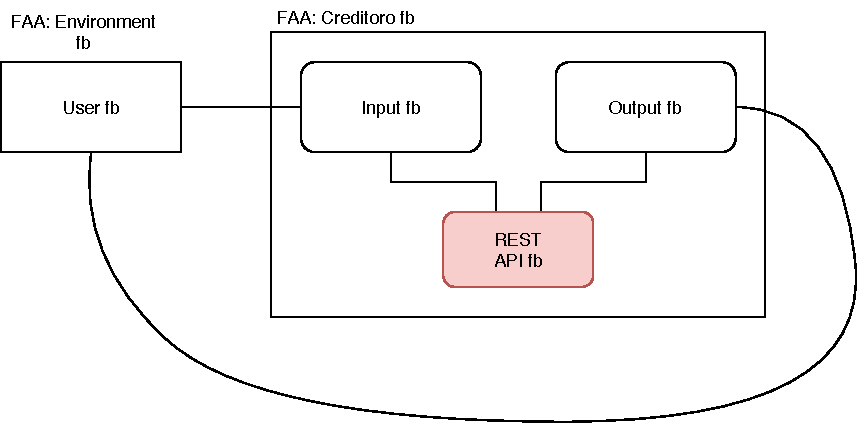
\includegraphics[scale=1]{figures/EAST-ADL/main.pdf}
\caption{EAST-ADL model - Main}
\label{fig:main}
\end{figure}